
%%%%%%%%%%%%%%%%%%%%%%% file typeinst.tex %%%%%%%%%%%%%%%%%%%%%%%%%
%
% This is the LaTeX source for the instructions to authors using
% the LaTeX document class 'llncs.cls' for contributions to
% the Lecture Notes in Computer Sciences series.
% http://www.springer.com/lncs       Springer Heidelberg 2006/05/04
%
% It may be used as a template for your own input - copy it
% to a new file with a new name and use it as the basis
% for your article.
%
% NB: the document class 'llncs' has its own and detailed documentation, see
% ftp://ftp.springer.de/data/pubftp/pub/tex/latex/llncs/latex2e/llncsdoc.pdf
%
%%%%%%%%%%%%%%%%%%%%%%%%%%%%%%%%%%%%%%%%%%%%%%%%%%%%%%%%%%%%%%%%%%%


%\documentclass{llncs}%[runningheads,a4paper]
\documentclass[runningheads,a4paper]{llncs}
\usepackage{llncsdoc}
\usepackage{times}
\usepackage{amssymb}
%\setcounter{tocdepth}{3}
\usepackage{graphicx}
\usepackage{amsmath}
\usepackage{color}
%\usepackage{mathrsfs}
%\usepackage{epstopdf}
%\usepackage{multirow}
%\usepackage{subfigure}
%\usepackage{hyperref}
%\usepackage{titlesec}
\usepackage{amssymb}
\usepackage{stmaryrd}
\usepackage{graphicx}
\usepackage{fancyvrb}
\usepackage{url}
\usepackage{fancyvrb}


\setcounter{secnumdepth}{4}



\begin{document}

\mainmatter  % start of an individual contribution

\title{A Study on Performance Comparison \\ of Structural Learning Algorithms \\ about Synthetic Pattern of Bayesian Network}

\author{Jae-seong Yoo$^{1}$, Baek-woon Yu$^{2}$ and Rae-hyun Chang$^{2}$}

\institute{$^{1}$Department of Computer Science and Engineering, Korea University, Republic of Korea\\$^{2}$Department of Brain and Cognitive Engineering, Korea University, Republic of Korea
}

\maketitle

\begin{abstract}
Bayesian networks(BN) are graphical models where nodes represent random variables and arrows represent probabilistic dependencies between them. And structure learning refers to a method of finding the structure when only know about variables. Many algorithms have been developed for this. Therefore, the purpose of these algorithms is to find the groundtruth correctly.

The Bayesian network can have many different shapes. In particular, as the number of nodes increases, the number of possible shapes increases exponentially. So should we measure performance for all shapes? It seems impossible to measure performance for all shapes.

However, if we have a somewhat stereotypical shapes, we will be able to do that. At least, we will be able to do these shapes. It is our goal to do this minimal thing.
\end{abstract}




\section{The Basics of Bayesian Network Structure Learning}

\subsection{Bayesian Network}
	
Bayesian networks(BN) are graphical models where nodes represent random variables and arrows represent probabilistic dependencies between them {\scriptsize{}(Kevin B. K. and Ann E. N., 2010)}.

A $n$-dimensional BN is a triple $B = (X, G, \Theta)$ where:

\begin{itemize}
	\item $X$ is a $n$-dimensional finite random vector each random variable $X_{i}$ ranges over by a finite domain $D_{i}$. Henceforward, we denote the joint domain by $D=\prod_{i=1}^{n}D_{i}$
	
	\item $G = (N, E)$ is a directed acyclic graph(DAG) with nodes $N = \{X_{1}, \cdots, X_{n}\}$ and edges $E$ representing direct dependencies between the variables.
	
	\item $\Theta$ encodes the parameters $\{\theta_{ijk}\}_{i\in1,\cdots,n, \, j\in D_{\Pi_{X_{i}}}, \, k\in D_{i}}$ of the network, where
	$$\theta_{ijk}=P_{B}\left(X_{i}=x_{ik} \, | \, \prod_{X_{i}}=\omega_{ij}\right),$$
	
	$\Pi_{X_{i}}$ denotes the set of parents of $X_{i}$ in $G$, $D_{\Pi_{X_{i}}}$ denotes the joint domain of the variables in $\Pi_{X_{i}, \, x_{ik}}$ is the $k$-th value of $X_{i}$ and $\omega_{ij}$ is the $j$-th configuration of $\Pi_{X_{i}}$.
\end{itemize}

\begin{figure}
	\centering
	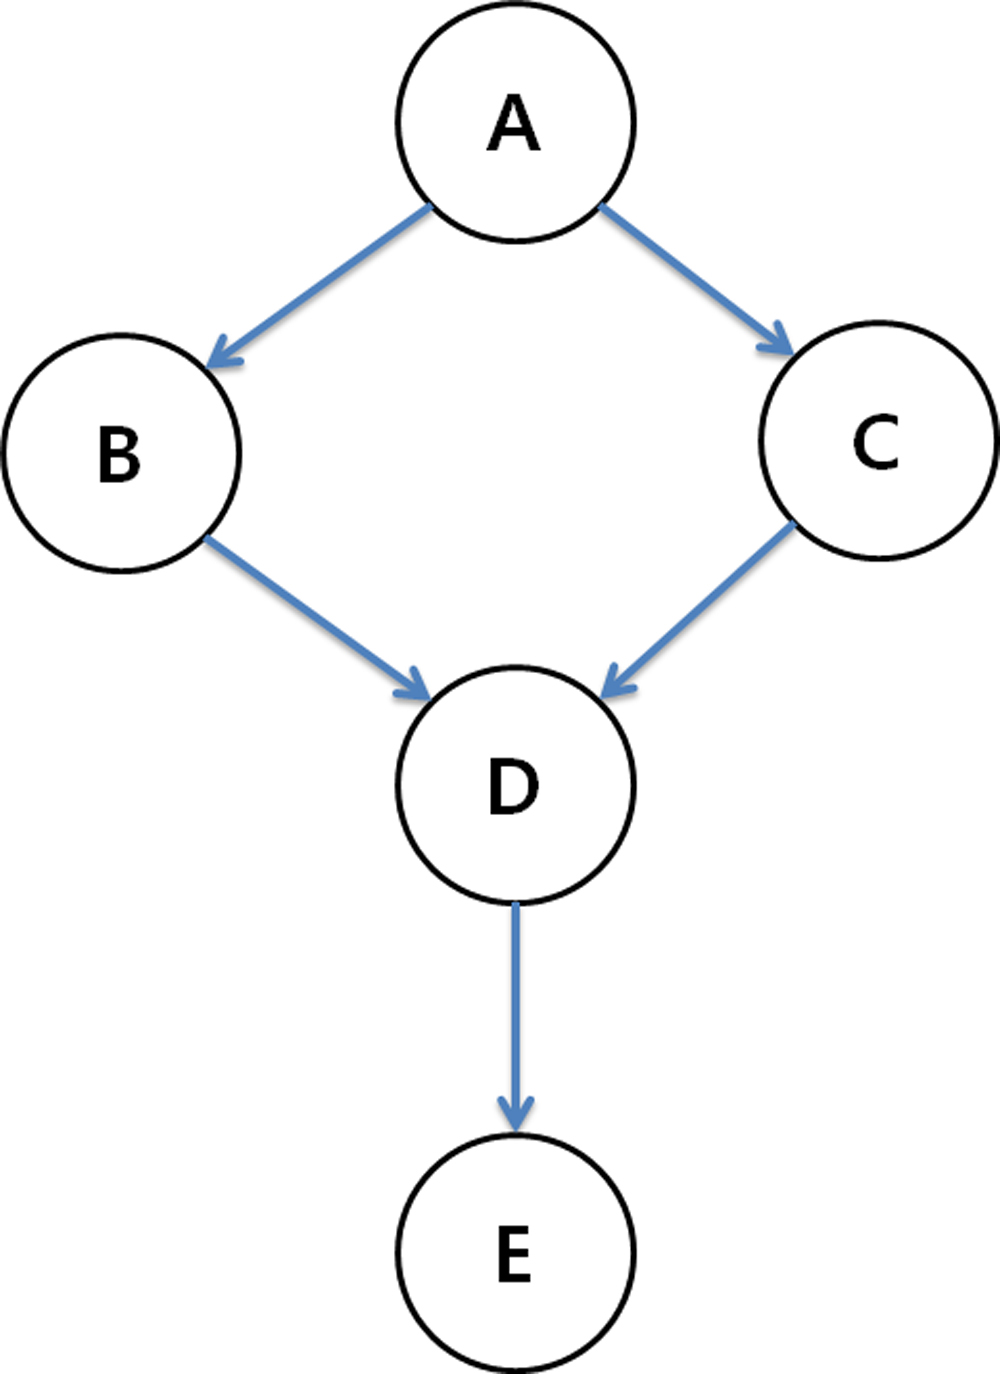
\includegraphics[height=100pt]{images/image01}
	\caption{\footnotesize{$P(A,B,C,D,E)=P(A)P(B|A)P(C|A)P(D|B,C)P(E|D)$}}
\end{figure}	

A BN defines a unique joint probability distribution over $X$ given by
$$P_{B}(X_{1},\cdots,X_{n})=\prod_{i=1}^{n}P_{B}\left(X_{i} \, | \, \prod_{X_{i}}\right).$$

\begin{itemize}
	\item A BN encodes the independence assumptions over the component random variables of $X$.
	
	\item An edge $(j, i)$ in $E$ represents a direct dependency of $X_{i}$ from $X_{j}$.
	
	\item The set of all Bayesian networks with $n$ variables is denotes by $B_{n}$.
\end{itemize}





\subsection{Bayesian Network Structure Learning}

The problem of learning a BN given data $T$ consists of finding the BN that best fits the data $T$. In order to quantify the fitting of a BN a scoring function $\phi$ is considered.

Learning a Bayesian network is as follows:

Given a data $T = \{y_{1}, \cdots, y_{n}\}$ and a scoring function $\phi$, the problem of learning a Bayesian network is to find a Bayesian network $B \in B_{n}$ that maximizes the value $\phi(B, T)$. {\scriptsize{}(Margaritis D., 2003, Marco S., 2010)}




\subsubsection{Constraint-based algorithms}

These algorithms learn the network structure by analyzing the probabilistic relations entailed by the Markov property of Bayesian networks with conditional independence tests and then constructing a graph which satisfies the corresponding d-separation statements. The resulting models are often interpreted as causal models even when learned from observational data {\scriptsize{}(Pearl J. 1988)}.

Grow-Shrink (GS) based on the Grow-Shrink Markov Blanket, the first (and simplest) Markov blanket detection algorithm used in a structure learning algorithm.
	
Incremental Association (IAMB) based on the Markov blanket detection algorithm of the same name, which is based on a two-phase selection scheme (a forward selection followed by an attempt to remove false positives).



\subsubsection{Score-based algorithms}

The main idea behind score-based learning is to optimize the degree of match between the generated network and the observations. {\scriptsize{}(Benjamin B. P., 2003)} These algorithms assign a score to each candidate Bayesian network and try to maximize it with some heuristic search algorithm. The search problem of identifying a Bayesian network that has a relative posterior probability greater than a given constant is NP-complete. {\scriptsize{}(D.M. Chickering, 1996)} Greedy search algorithms (such as hill-climbing or TABU search) are a common choice, but almost any kind of search procedure can be used.

Hill-Climbing (HC) a hill climbing greedy search on the space of the directed graphs. The optimized implementation uses score caching, score decomposability and score equivalence to reduce the number of duplicated tests.
	
Tabu Search (TABU) a modified hill climbing able to escape local optima by selecting a network that minimally decreases the score function.



\subsubsection{Hybrid algorithms}

Hybrid algorithms are combines the constraint-based and score-based.

Max-Min Hill-Climbing (MHHC) a hybrid algorithm which combines the Max-Min Parents and Children algorithm (to restrict the search space) and the Hill-Climbing algorithm (to find the optimal network structure in the restricted space).
	
Restricted Maximization (RSMAX2) a more general implementation of the Max-Min Hill-Climbing, which can use any combination of constraint-based and score-based algorithms.





\section{Varying topologies and number of nodes}


According to Robinson, R. W. (1973), the number of DAGs may be computed by the recurrence relation as shown below.
$$a_{n}=\sum_{k=1}^{n}(-1)^{k-1}\left(\begin{array}{c}
n\\
k
\end{array}\right)2^{k(n-k)}a_{n-k}$$

In other words, the number of DAGs on n labeled vertices, for n = 0, 1, 2, 3, … (without restrictions on the order in which these numbers appear in a topological ordering of the DAG) is 1, 1, 3, 25, 543, 29281, 3781503, $\cdots$.
These exponentially increasing numbers makes difficulties to check performance of each algorithms for structure learning.


Meanwhile, Eitel J. M. L., (2008) proposed a formal DAG model as \textbf{Fig. 2.}.

\begin{figure}[!h]
	\centering
	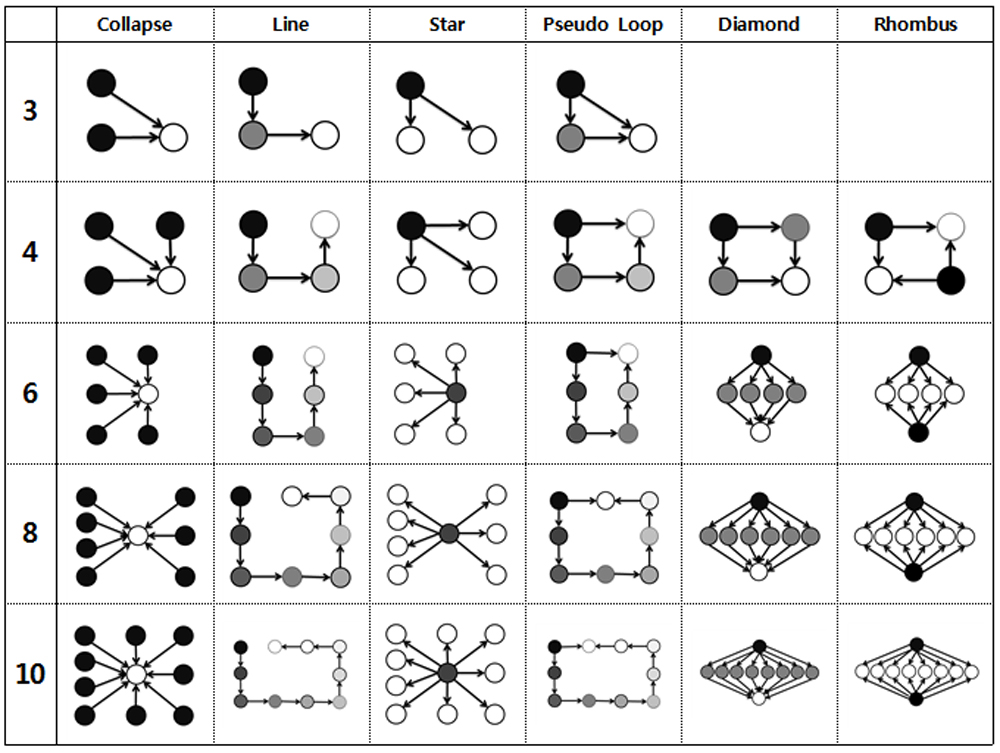
\includegraphics[height=200pt]{images/Topologies}
	\caption{\footnotesize{Bayesian Networks with varying topologies and number of nodes}}
\end{figure}	

If one node has plurality of parent nodes, then this form called \underline{Collapse}.

Multiple node bite the tail of the tail, then this form called \underline{Line}.

If one node has plurality of child node, then this form called \underline{Star}.

The description of the \underline{Pseudo Loop} is a little complicated. At first, drew a line form. And next, root node has depended on the very last child node. Then it called \underline{Pseudo Loop}. Actually loop does not have, it looks like a loop at glance.

A part of the top, one node has plurality of child node like Star form. And the bottom part, one node has plurality of parent node like Collapse form. If it connected, then it called \underline{Diamond}.

If two nodes has plurality of child node together, then it called \underline{Rhombus}.

Although it is difficult to evaluate the performance of the algorithm for all cases of the DAG model according to the number of nodes, but at least when the ground truth equals to \textbf{Fig. 2.}, we can compare.

The goal of our team is to compare the performance of the structure learning algorithm based on the above synthetic model and to confirm whether each algorithm learns the pattern of the synthetic model well.





\section{The Methodology of Performance Comparison}

\subsection{The Number of Graphical Errors in Learnt Structure}

The comparison methodology used in this paper is similar to the method used in X.-w. Chen \emph{et al.} (2006). The existence of the known network structures allows us to define three important terms which indicate the performance of the algorithm (in terms of the number of graphical errors in the learnt structure).

\begin{description}
	\item[C (Correct Arcs)] Edges present in the original network and in the learnt network structure.
	
	\item[M (Missing Arcs)] Edges present in the original network but not in the learnt network structure.
	
	\item[WO (Wrongly Oriented Arcs)] Edges present in the learnt network structure, but having opposite orientation when compared with the corresponding edge in the original network structure.
	
	\item[WC (Wrongly Corrected Arcs)] Edges not present in the original network but included in the learnt network structure.
\end{description}

\begin{center}
	\begin{tabular}{c|l|c|c|c}
		\hline 
		& & \textbf{Target Network} & \textbf{Learnt Network} & \textbf{Direction}\tabularnewline
		\hline 
		\textbf{\textcolor{blue}{C}} & (Correct Arcs) & exist & exist & correct\tabularnewline
		\textbf{\textcolor{blue}{M}} & (Missing Arcs) & exist & \textcolor{red}{not exist} & \tabularnewline
		\textbf{\textcolor{blue}{WO}} & (Wrongly Oriented Arcs) & exist & exist & \textcolor{red}{wrong}\tabularnewline
		\textbf{\textcolor{blue}{WC}} & (Wrongly Corrected Arcs) & not exist & \textcolor{red}{exist} & \tabularnewline
		\hline 
	\end{tabular}
\end{center}





\subsection{Network Scores}

The values of the BDe, the Log-likelihood (LL), the AIC, and the BIC are metrics for the learned networks. {\scriptsize{}(Alexandra M. C., 2009)} These measures can offer an idea of the quality of the networks from different points of view. In all four cases, the higher the value of the metric, the better the network. {\scriptsize{}(D. Heckerman \emph{et al.}, 1995, Silvia A. \emph{et al.}, 2004)}.

\begin{center}\rule[0.5ex]{0.9\columnwidth}{1pt}\end{center}

\begin{description}
	\item[BDe]
	$BDe(B,T) = P(B,T)=P(B)\times\prod_{i=1}^{n}\prod_{j=1}^{q_{i}}(\frac{\Gamma(N'_{ij})}{\Gamma(N_{ij}+N'_{ij})}\times\prod_{k=1}^{r_{i}}\frac{\Gamma(N_{ijk}+N'_{ijk})}{\Gamma(N'_{ijk})})$
\end{description}

\begin{center}\rule[0.5ex]{0.9\columnwidth}{1pt}\end{center}
$$\phi(B|T) = LL(B|T) - f(N)|B|,$$
$$LL(B|T)=\sum_{i=1}^{n}\sum_{j=1}^{q_{i}}\sum_{k=1}^{r_{i}}N_{ijk}\log(\frac{N_{ijk}}{N_{ij}}).$$

\begin{description}
	\item[Log-Likelihood(LL)] If $f(N) = 0$, we have the \textbf{LL} score.
	
	\item[AIC] If $f(N) = 1$, we have the \textbf{AIC} scoring function:
	
	\item[BIC] If $f(N) = \frac{1}{2} \log(N)$, we have the \textbf{BIC} score.
\end{description}

\begin{center}\rule[0.5ex]{0.9\columnwidth}{1pt}\end{center}





\section{Simulation}

In this project, depending on the topology like Fig. 2., after create a set of models of the number of nodes to 3, 4, 6, 8, 10 pieces, and simulate with following restrictions.

\begin{itemize}
	\item Cardinality was limited to two. It means, all variables are binary data.
	
	\item  The probability value was set by Uniform distribution with minimum value is 0 and maximum value is 1. This way, we can make a more stochastic interpretation.
	
	\item All experiments are repeated 100 times. Because it is to avoid the consequences of coincidence.
	
	\item Constraint-based Learning Algorithms often makes undirected arcs. So, this has been excluded from comparison.
\end{itemize}
  
{}\
  
	\begin{figure}
		\centering
		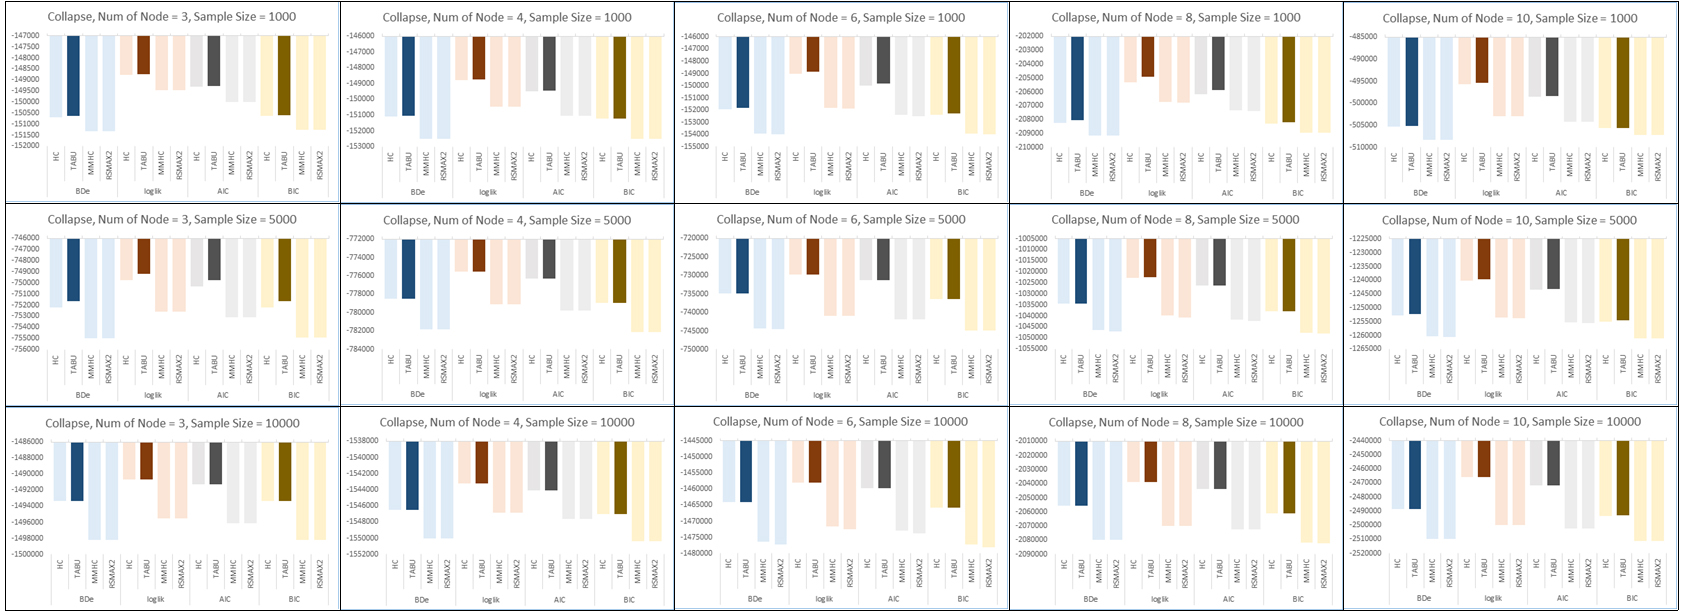
\includegraphics[width=280pt, height=95pt]{images/01_Collapse_Score}
		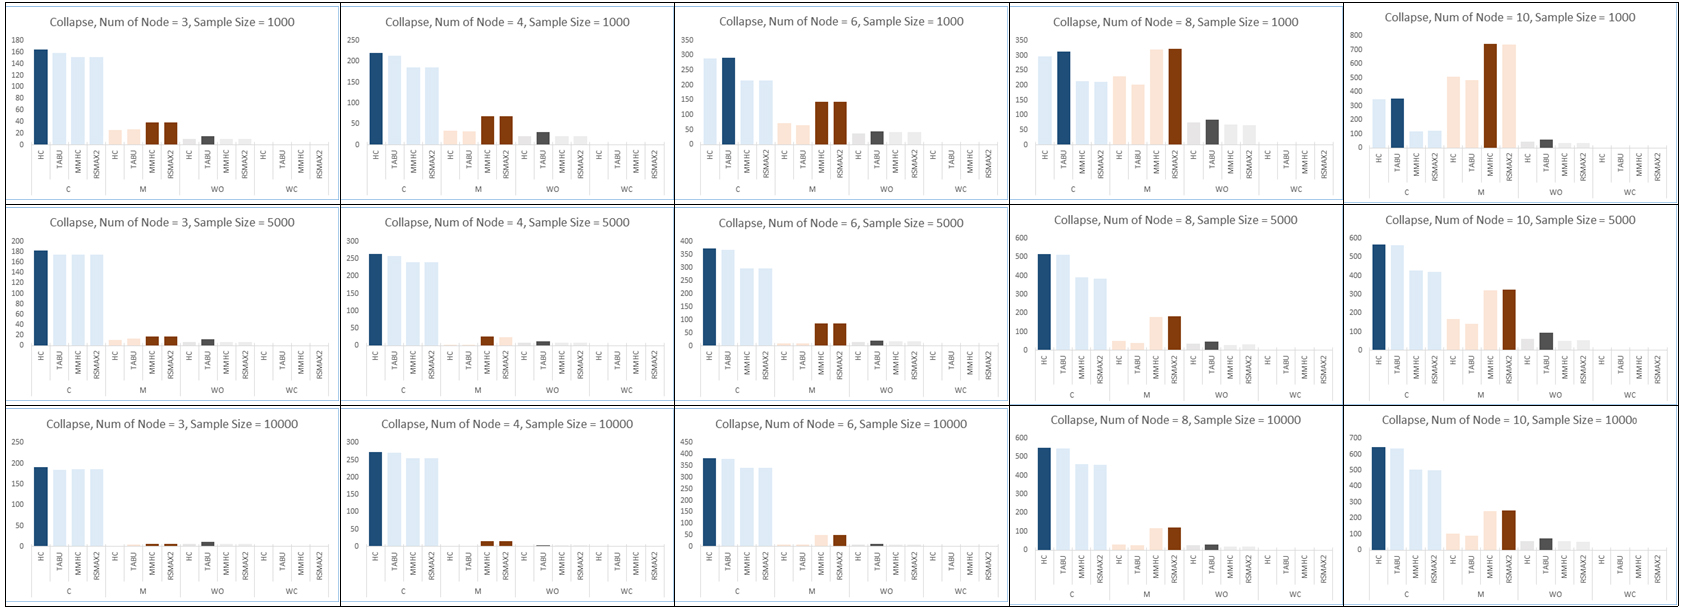
\includegraphics[width=280pt, height=95pt]{images/01_Collapse_Arcs}
		\caption{Comparison of scores(top) and correct arcs(bottom) via Collapse}
		{
			\begin{itemize}
				\item According to scores, TABU $>$ HC $>>>$ MMHC = RSMAX2
				
				\item According to correct arcs, HC $>$ TABU $>$ MMHC = RSMAX2
					
				\item Therefore, {\color{red}HC = TABU $>>>$ MMHC = RSMAX2}
			\end{itemize}
		}
	\end{figure}
	



	\begin{figure}
		\centering
		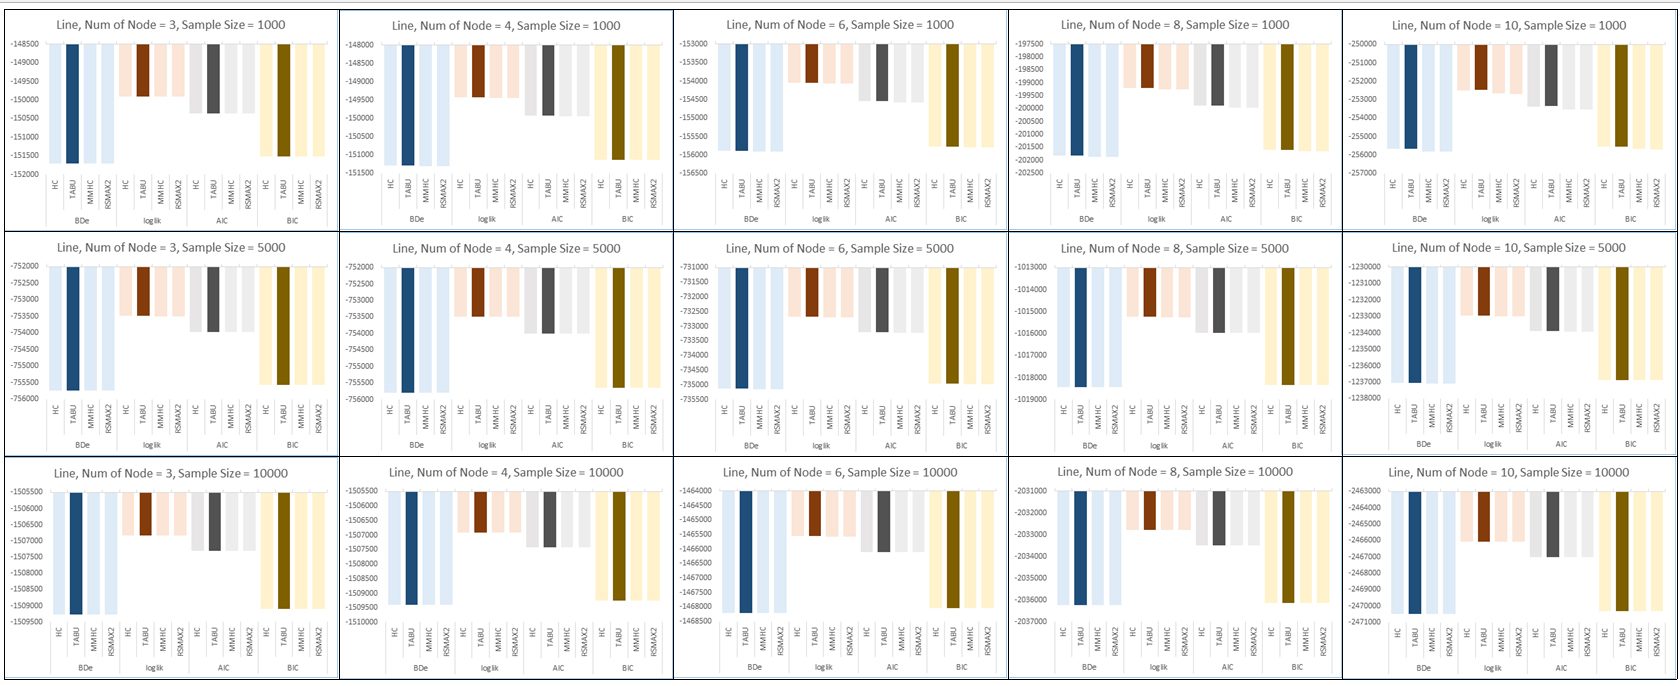
\includegraphics[width=280pt, height=95pt]{images/02_Line_Score}
		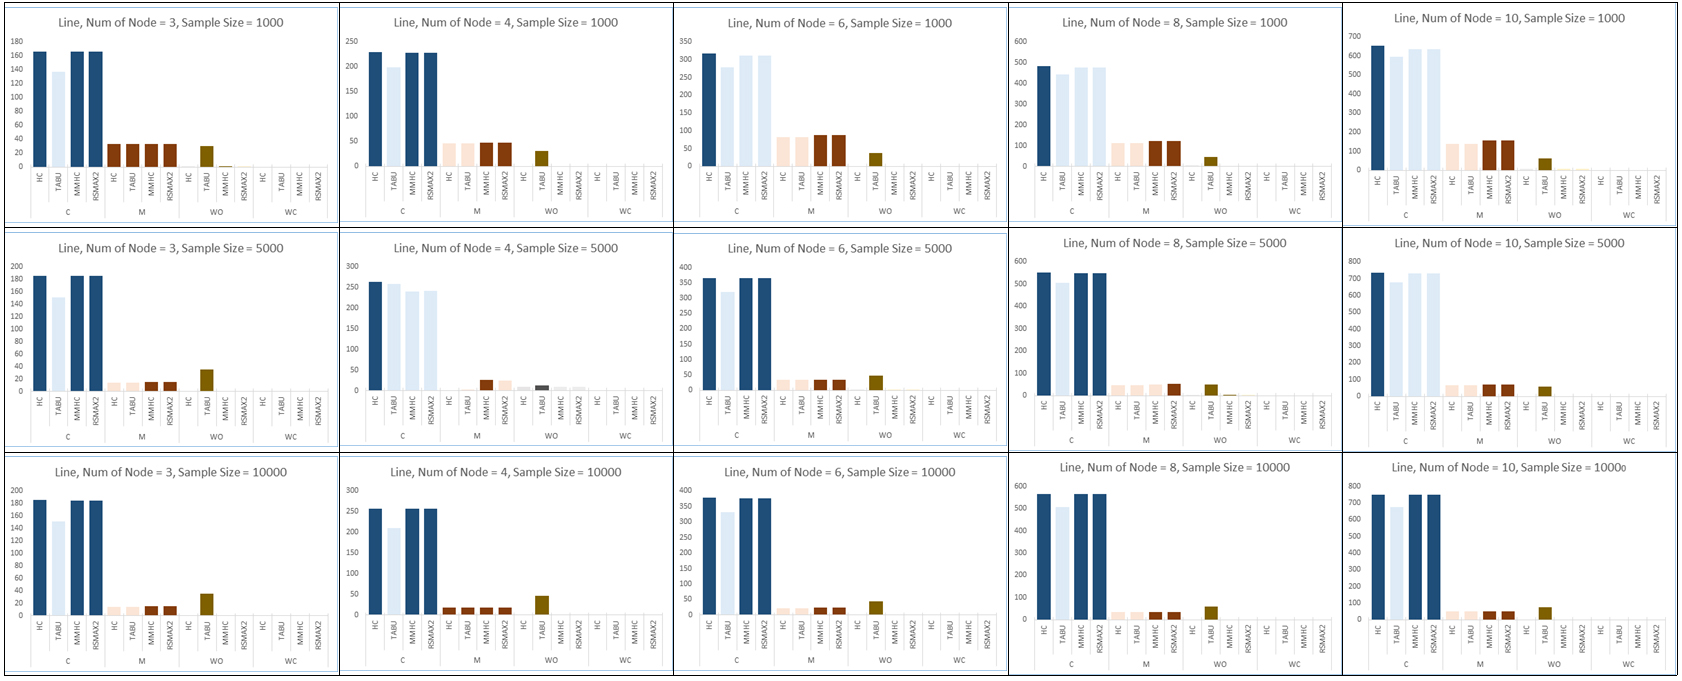
\includegraphics[width=280pt, height=95pt]{images/02_Line_Arcs}
		\caption{Comparison of scores(top) and correct arcs(bottom) via Line}
		{
			\begin{itemize}
				\item According to scores, TABU $>$ HC = MMHC = RSMAX2
				
				\item According to correct arcs, HC = MMHC = RSMAX2 $>>>$ TABU
				
				\item Therefore, {\color{red}HC = MMHC = RSMAX2 $>>>$ TABU}
			\end{itemize}
		}
	\end{figure}




	\begin{figure}
		\centering
		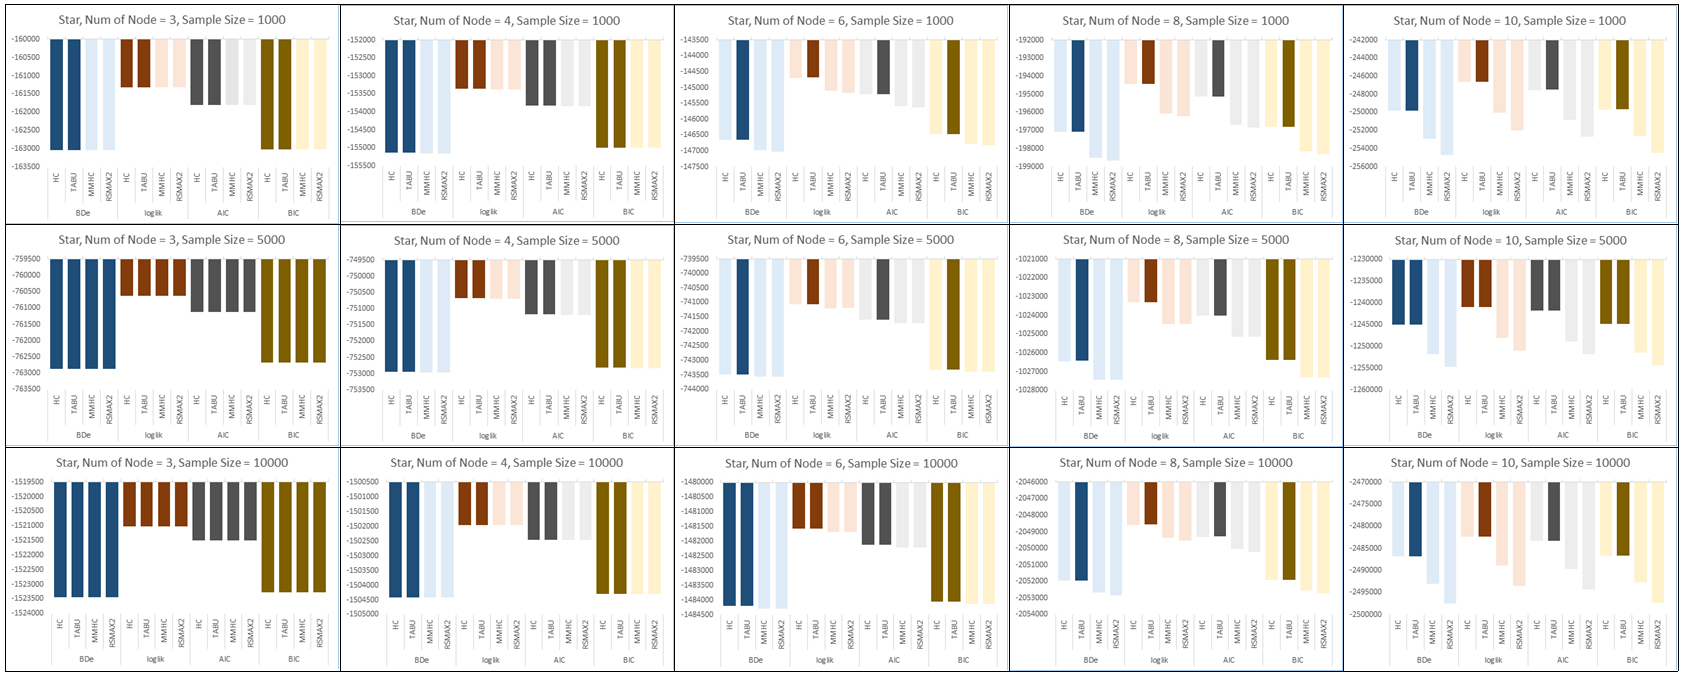
\includegraphics[width=280pt, height=95pt]{images/03_Star_Score}
		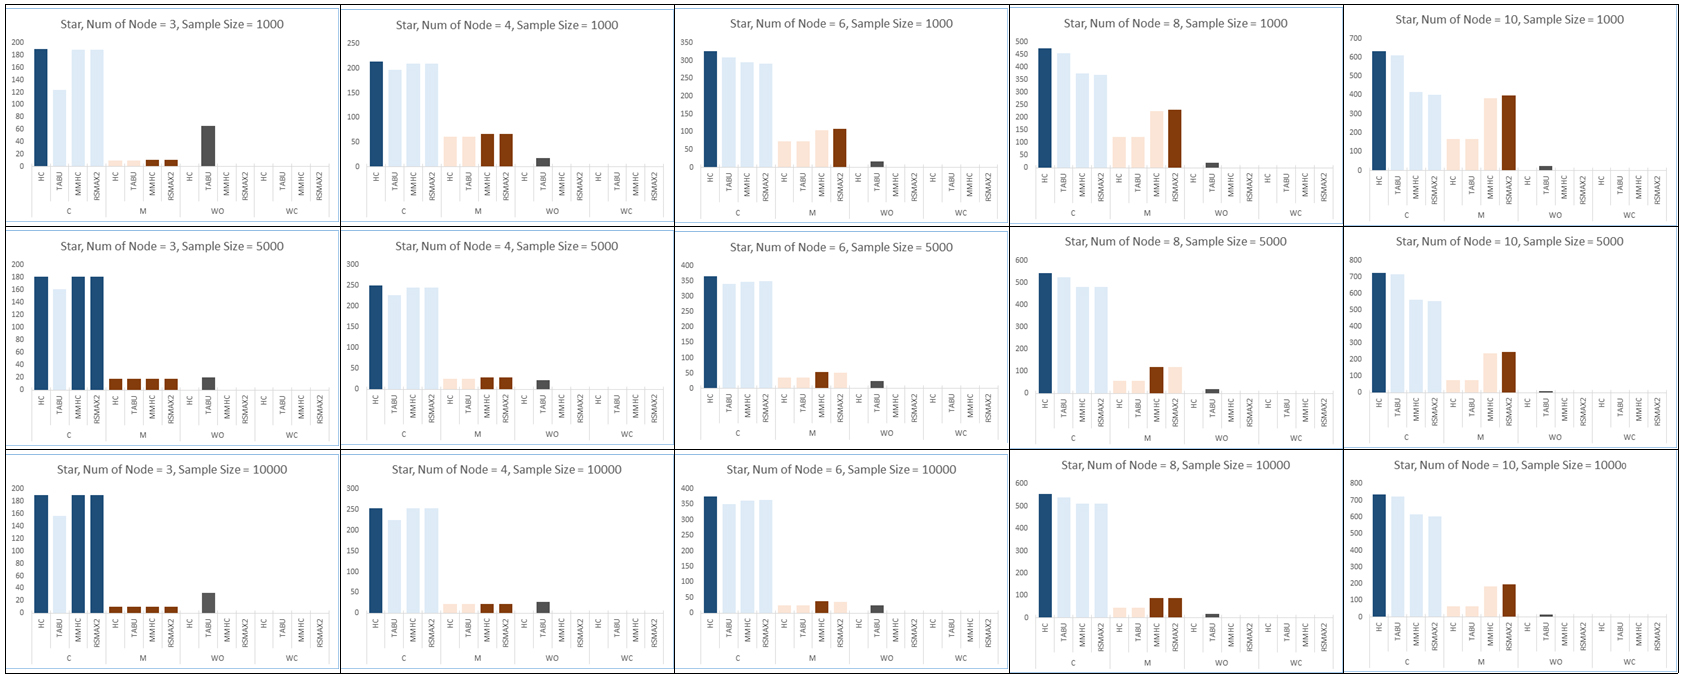
\includegraphics[width=280pt, height=95pt]{images/03_Star_Arcs}
		\caption{Comparison of scores(top) and correct arcs(bottom) via Star}
		{
			\begin{itemize}
				\item According to scores, HC = TABU $>$ MMHC = RSMAX2
				
				\item According to correct arcs, HC $>$ TABU = MMHC = TABU
				
				\item Therefore, {\color{red}HC $>$ TABU = MMHC = RSMAX2}
			\end{itemize}
		}
	\end{figure}	




	\begin{figure}
		\centering
		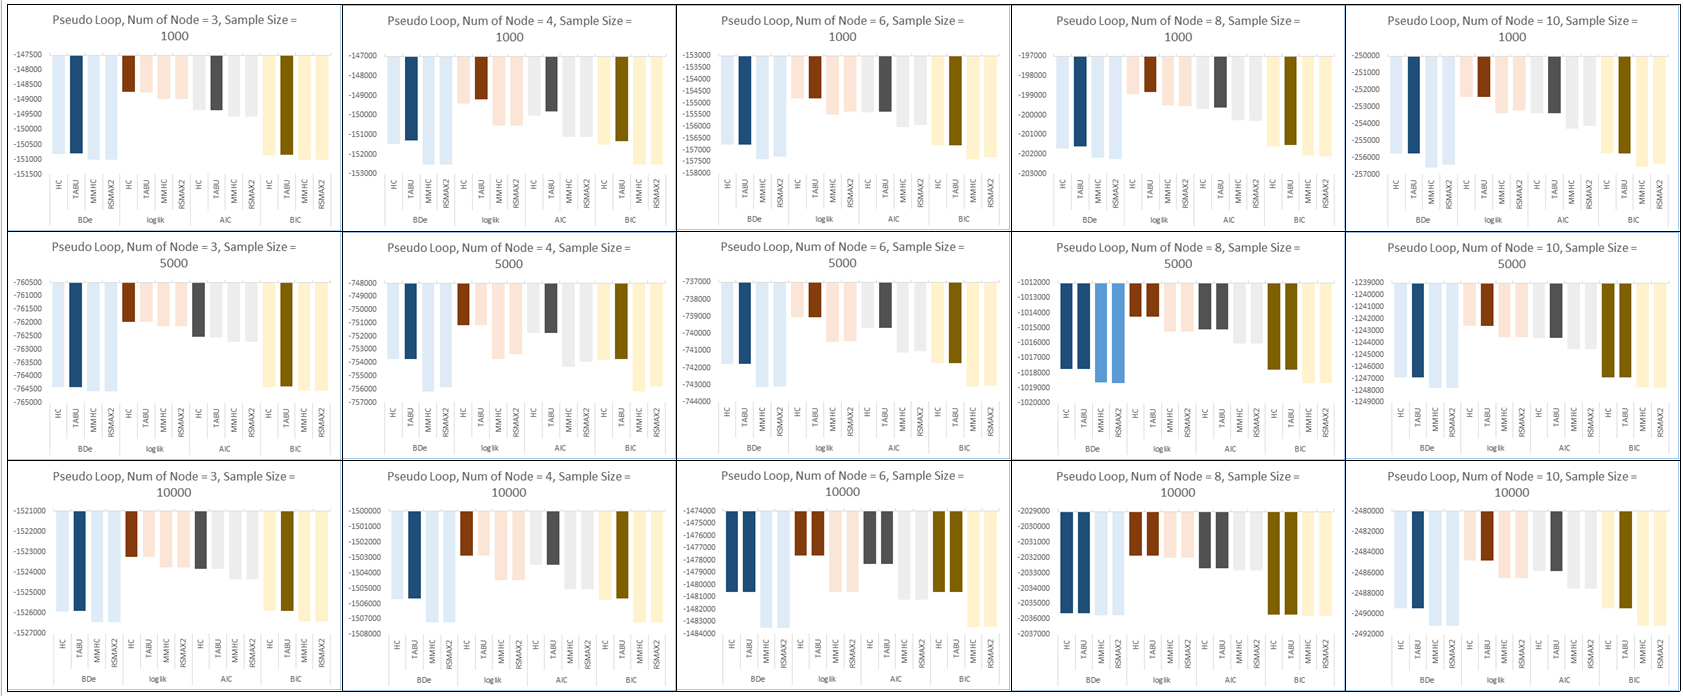
\includegraphics[width=280pt, height=95pt]{images/04_PseudoLoop_Score}
		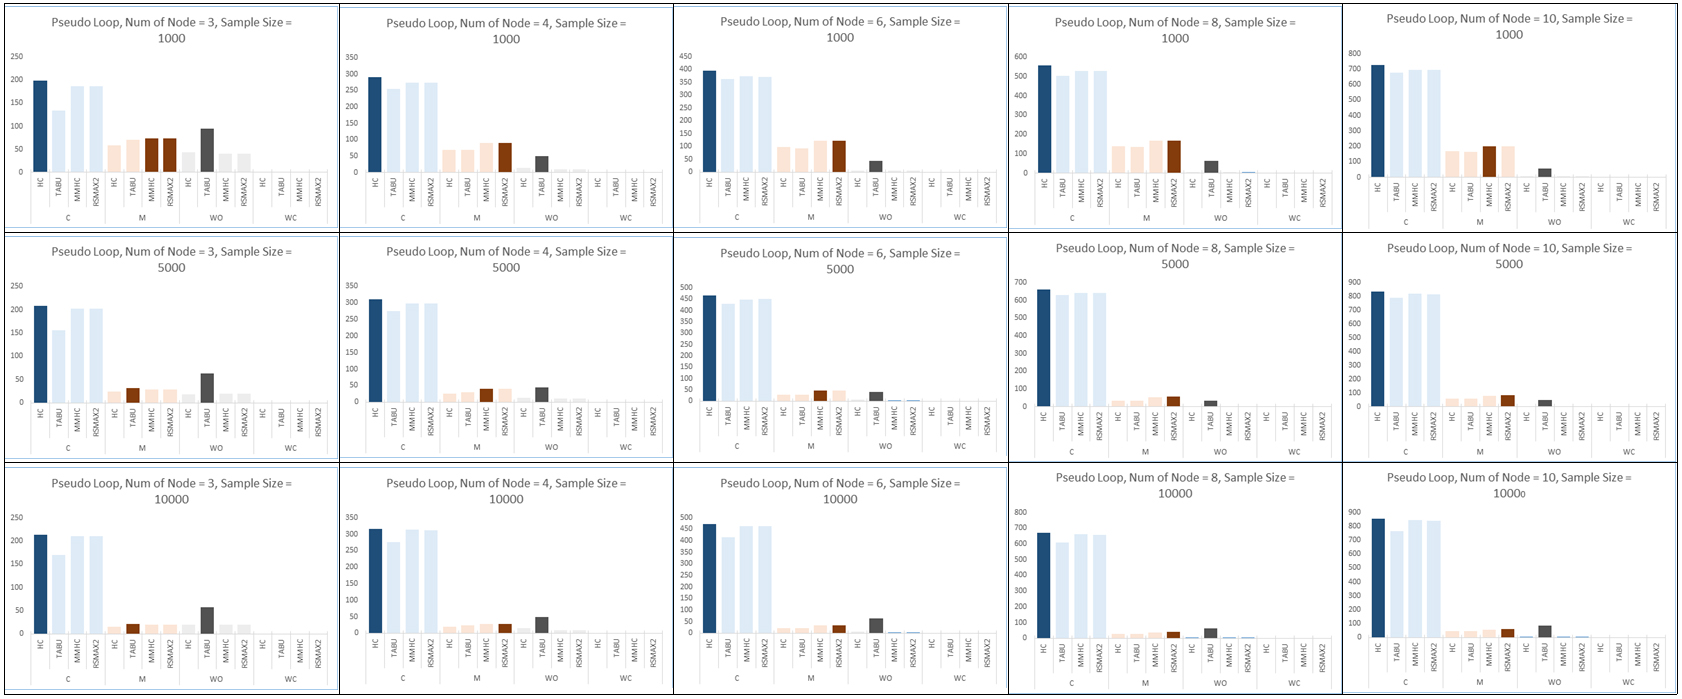
\includegraphics[width=280pt, height=95pt]{images/04_PseudoLoop_Arcs}
		\caption{Comparison of scores(top) and correct arcs(bottom) via Pseudo Loop}
		{
			\begin{itemize}
				\item According to scores, TABU $>$ HC $>$ MMHC $>$ RSMAX2
				
				\item According to correct arcs, HC $>$ MMHC = RSMAX2 $>>>$ TABU
				
				\item Therefore, {\color{red}HC $>>>$ TABU = MMHC = RSMAX2}
			\end{itemize}
		}
	\end{figure}	




	\begin{figure}
		\centering
		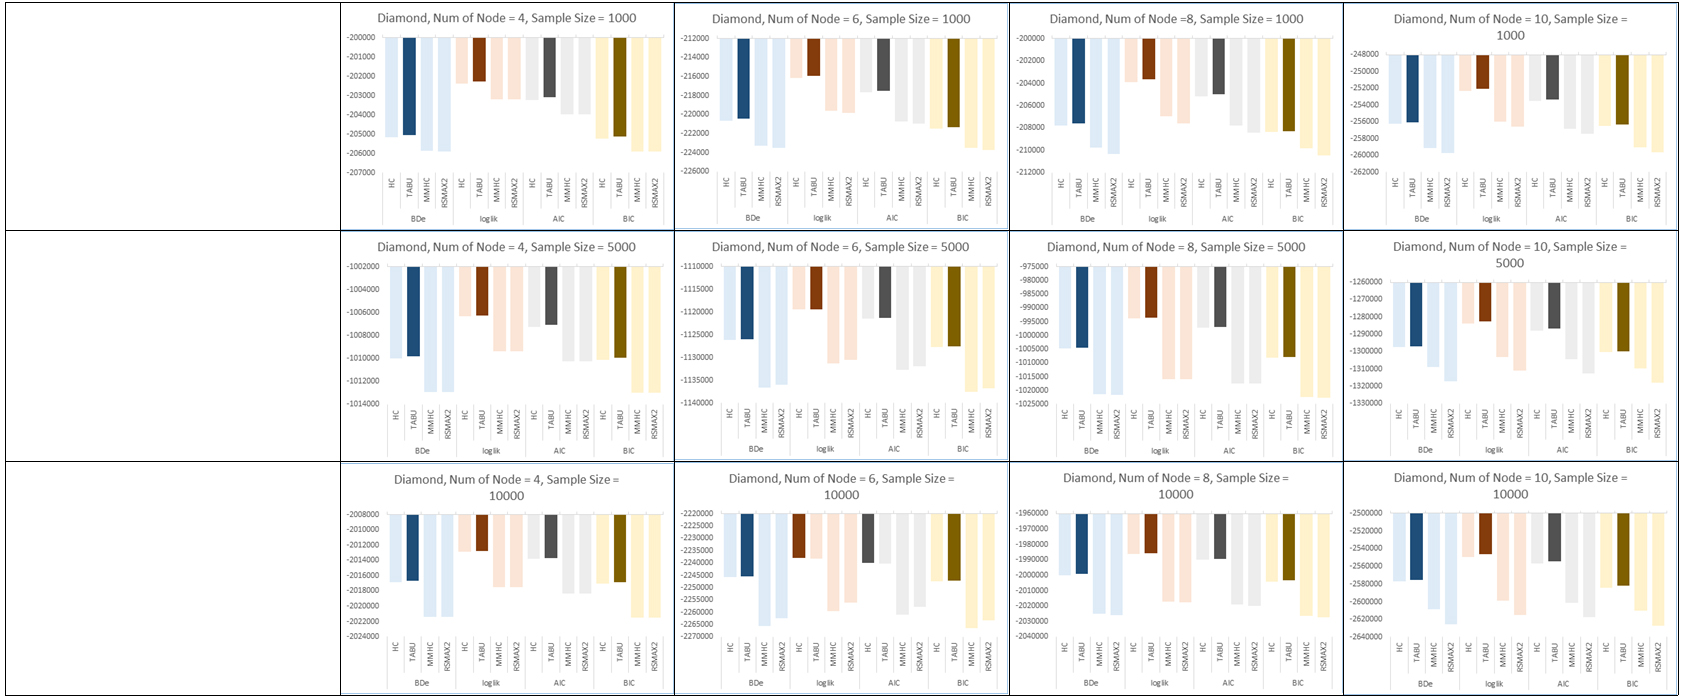
\includegraphics[width=280pt, height=95pt]{images/05_Diamond_Score}
		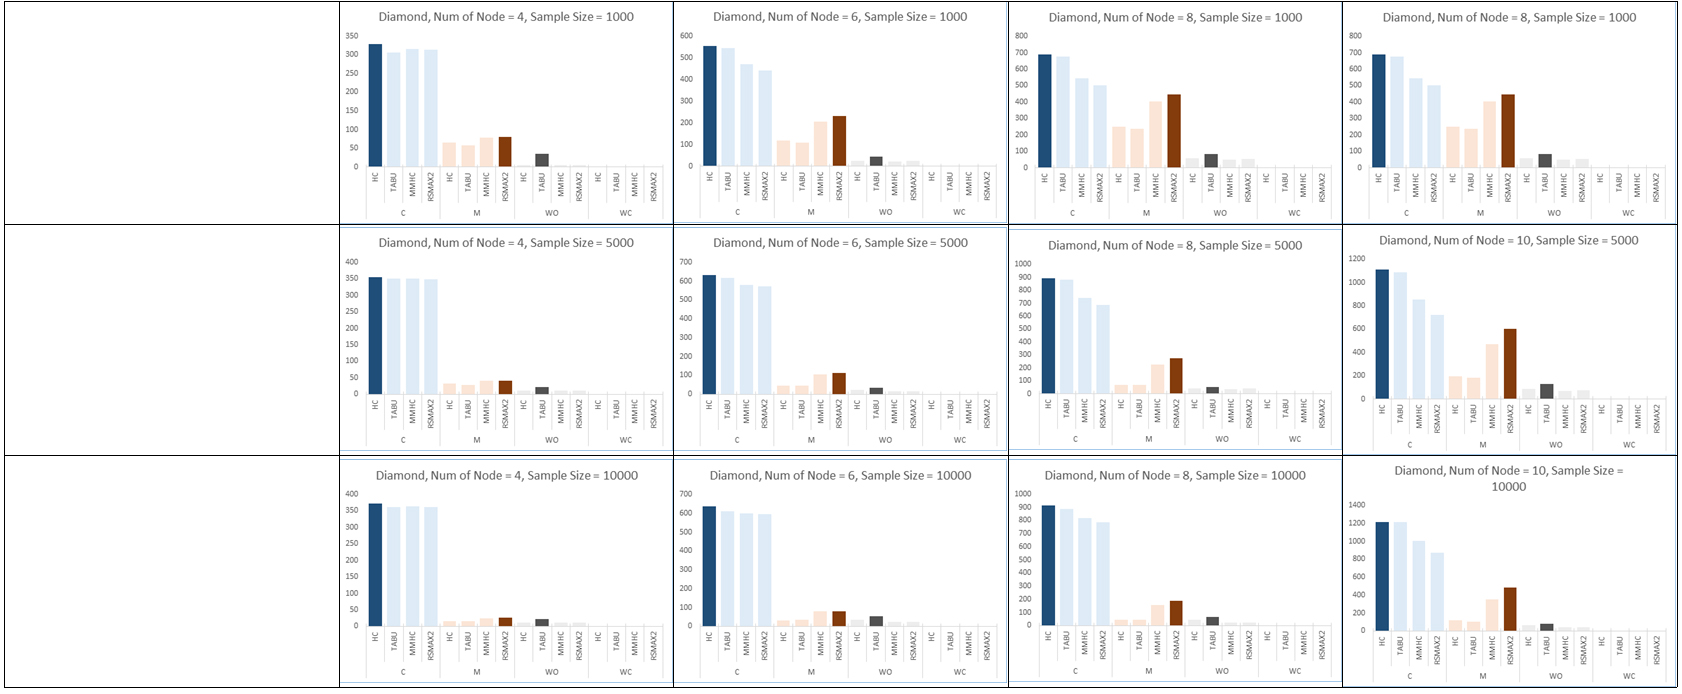
\includegraphics[width=280pt, height=95pt]{images/05_Diamond_Arcs}
		\caption{Comparison of scores(top) and correct arcs(bottom) via Diamond}
		{
			\begin{itemize}
				\item According to scores, TABU $>$ HC $>>>$ MMHC $>$ RSMAX2
				
				\item According to correct arcs, HC $>$ TABU $>>>$ MMHC = RSMAX2
				
				\item Therefore, {\color{red}HC = TABU $>>>$ MMHC $>$ RSMAX2}
			\end{itemize}
		}
	\end{figure}	




	\begin{figure}
		\centering
		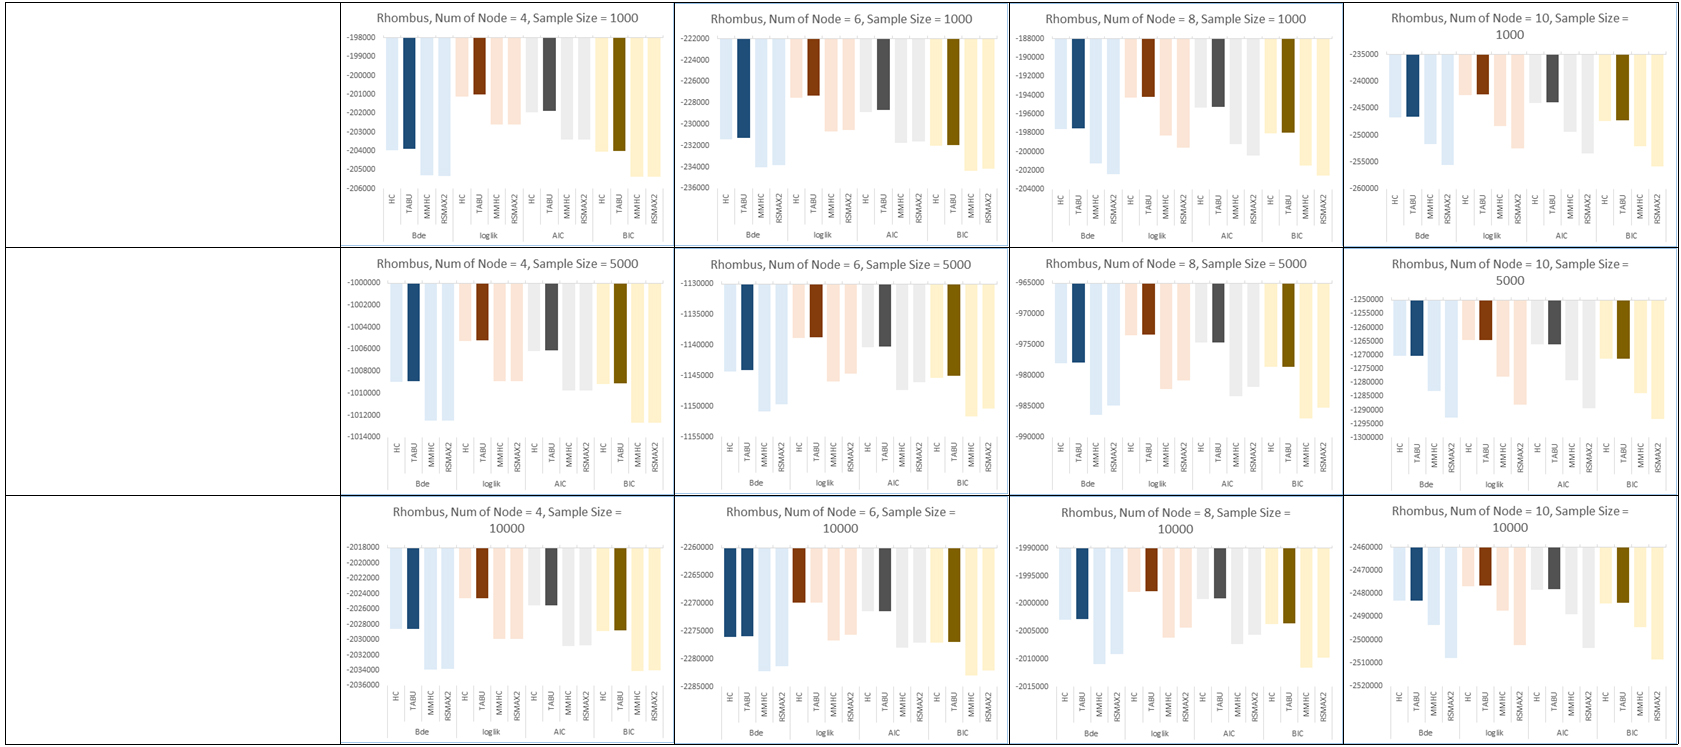
\includegraphics[width=280pt, height=95pt]{images/06_Rhombus_Score}
		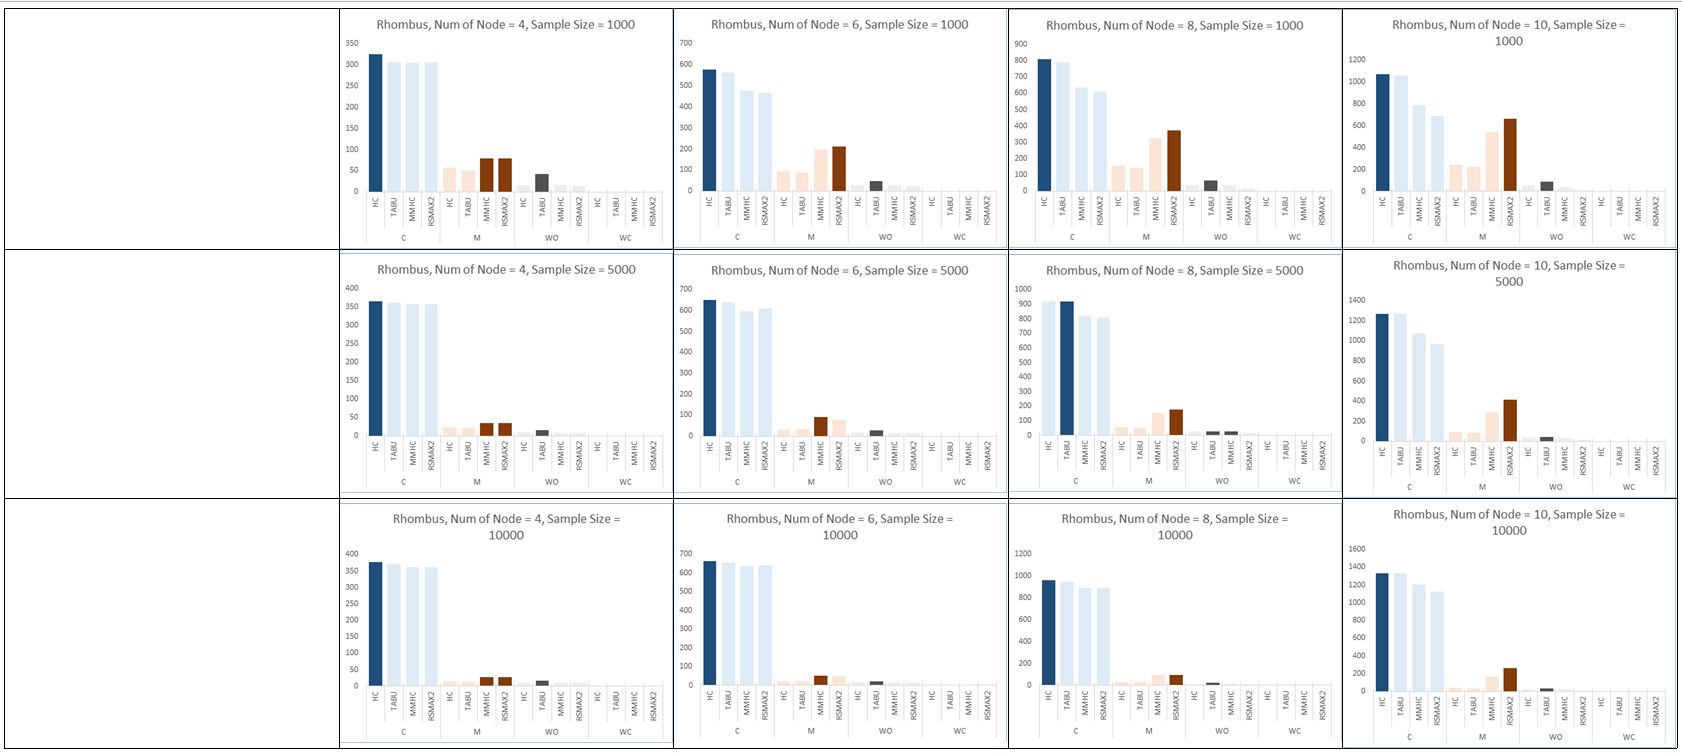
\includegraphics[width=280pt, height=95pt]{images/06_Rhombus_Arcs}
		\caption{Comparison of scores(top) and correct arcs(bottom) via Rhombus}
		{
			\begin{itemize}
				\item According to scores, TABU $>$ HC $>>>$ MMHC $>$ RSMAX2
				
				\item According to correct arcs, HC $>$ TABU $>>>$ MMHC = RSMAX2
				
				\item Therefore, {\color{red}HC = TABU $>>>$ MMHC $>$ RSMAX2}
			\end{itemize}
		}
	\end{figure}	



\newpage{}

\section{Result}

	Results of compare the performance of each algorithm according to topologies like below.
	
	\begin{description}
		\item[Collapse:] {\color{red}HC = TABU} $>>>$ MMHC = RSMAX2
		
		\item[Line:] {\color{red}HC = MMHC = RSMAX2} $>>>$ TABU
		
		\item[Star:] {\color{red}HC} $>$ TABU = MMHC = RSMAX2
		
		\item[Pseudo Loop:] {\color{red}HC} $>>>$ TABU = MMHC = RSMAX2
		
		\item[Diamond:] {\color{red}HC = TABU} $>>>$ MMHC $>$ RSMAX2
		
		\item[Rhombus:] {\color{red}HC = TABU} $>>>$ MMHC $>$ RSMAX2
	\end{description}	 

Now, if we have a guess of groundtruth, we can select an algorithm for structure learning easily. Perhaps, this project suggests that Hill-Climbing is a good choice. However, when the many M, WO, WC is fatal, it will be able to try to consider the selection of hybrid algorithm. Hybrid algorithm compared to Score-based algorithm is found to be that draw the arc more conservative. This makes not only C is often less missing arcs, but also WO and WC is drawn very small. It seems to use when WO and WC are fatal. Especially MMHC and RSMAX2 for "Line" seems to be advantageous

In future study, it can be to increase the number of node topology, to complex topology, to less sample size, or to increase the cardinality.

In this project, the probability when defining the relationship between the probability gave arbitrarily values on U(0, 1). But it is possible to confirm the relationship when given "sequential" probability in future study.



\section*{Test Codes}
\url{https://github.com/JaeseongYoo/PatternRecognition}



\section*{Bibliography}
\bibliographystyle{splncs03}
%\bibliography{reference}

\begin{bibliography}{99}
	\addcontentsline{toc}{chapter}{Bibliography}
	\begin{enumerate}
		%\bibitem{ref1} 저자 (0000), 제목, \emph{저널}, Vol. 18, No. 3, 543-553.
		
		\bibitem{ref1} Alexandra M. C., (2009), Scoring functions for learning Bayesian networks \emph{Inesc-id Tec. Rep.}
		
		\bibitem{ref1} Beinlich I., Suermondt H. J., Chavez R. M. and Cooper G. F., (1989), The ALARM monitoring system: A case study with two probabilistic inference techniques for belief networks, \emph{Proceedings of the 2nd European Conference on Artificial Intelligence in Medicine}, 247-256.
		
		\bibitem{ref1} Binder J., Koller D., Russell S. and Kanazawa K., (1997), Adaptive probabilistic networks with hidden variables, \emph{Machine Learning}, Vol. 29, No. 2-3, 213-244.
		
		\bibitem{ref1} Daly R. and Shen Q., (2007), Methods to accelerate the learning of Bayesian network structures, \emph{Proceedings of the 2007 UK Workshop on Computational Intelligence, Imperial College, London.}
				
		\bibitem{ref1} D. M. Chickering, (1996), Learning Bayesian networks is NP-complete, \emph{Learning from Data: Artificial Intelligence and Statistics V, Springer Verlag.}
		
		\bibitem{ref1} Eitel J. M. L., (2008), An Information-geometric approach to learning Bayesian network topologies from data, \emph{Innovations in Bayesian Networks Studies in Computational Intelligence}, Vol. 156, 187-217.
			
		\bibitem{ref1} Kevin B. K. and Ann E. N., (2010), \emph{Bayesian Artificial Intelligence, 2nd Edition}, CRC Press.
			
		\bibitem{ref1} Marco S., (2010), Learning Bayesian networks with the bnlearn R package, \emph{Journal of Statistical Software}, Vol. 35, Issue 3.
		
		\bibitem{ref1} Margaritis D., (2003), Learning Bayesian network model structure from data, \emph{Ph.D. thesis, School of Computer Science, Carnegie-Mellon University, Pittsburgh, PA}, Available as Technical Report CMU-CS-03-153.
		
		\bibitem{ref1} Pearl J., (1988), \emph{Probabilistic Reasoning in Intelligent Systems: Networks of Plausible Inference}, Morgan Kaufmann.
		
		\bibitem{ref1} Robinson, R. W. (1973), Counting labeled acyclic digraphs, \emph{New Directions in the Theory of Graphs, Academic Press}, pp. 239–273.
		
		\bibitem{ref1} X.-w. Chen, G. Anantha, and X. Wang, (2006), An effective structure learning method for constructing gene networks, \emph{Bioinformatics}, Vol. 22, 1367-1374.
	\end{enumerate}
\end{bibliography}



\end{document}



